\begin{kbox}{9. 随机过程维度的物理意义(补充)}
    \textbf{为什么会有“一维”和“二维”之分?}
    \begin{itemize}
        \item \textbf{一维 PDF ($f_1$) —— 看“切片”(静态)}:
        固定某一时刻 $t$ 观察。它决定了信号的\textbf{均值}和\textbf{方差}(即平均功率、直流/交流分量)。
        \item \textbf{二维 PDF ($f_2$) —— 看“关联”(动态)}:
        固定两个时刻 $t_1, t_2$ 观察。它包含了\textbf{相关性}信息。不看二维就无法定义自相关函数 $R(\tau)$,也就无法得到功率谱密度 (PSD)。
    \end{itemize}
    
    \tcbline
    
    \textbf{为什么通信中主要关注 1维 和 2维?}
    虽然理论上随机过程有无限维 ($n$维),但在工程应用中:
    \begin{enumerate}
        \item \textbf{高斯过程的特性}:由其 1维(均值)和 2维(自相关/协方差)特性\textbf{完全决定}。即知道了前两维,就确定了整个随机过程。
        \item \textbf{广义平稳 (WSS)}:工程主要处理 WSS 过程,其定义标准仅依赖于均值(1维特性)和自相关函数(2维特性)。
    \end{enumerate}
\end{kbox}

\begin{examplebox}{例 3.2(1):求自相关函数 (详细推导版)}
    \textbf{题目描述}:已知随机过程 $\xi(t)$ 的功率谱密度 $P_\xi(f)$ 如图所示(三角形波 + 直流冲激),求自相关函数 $R(\tau)$。
        \begin{center}
            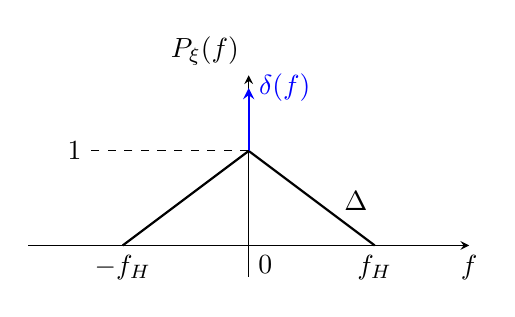
\begin{tikzpicture}[>=stealth, scale=0.8]
                % --- 坐标轴调整 ---
                \draw[->] (-3.5,0) -- (3.5,0) node[below] {$f$};
                % [修改点1]: 将纵轴标签移到左上方,避免与右侧的 delta(f) 标签打架
                \draw[->] (0,-0.5) -- (0,2.7) node[above left] {$P_{\xi}(f)$};
                % --- 三角波 ---
                \draw[thick] (-2,0) -- (0,1.5) -- (2,0);
                % [修改点2]: 将三角符号向右移动 (x坐标从 1.2 改为 1.7)
                \node at (1.7, 0.7) {$\Delta$};
                % --- 直流冲击 delta(f) ---
                % 保持粗线条和蓝色,绘制在坐标轴上方,标签在右侧
                \draw[->, thick, blue] (0,1.5) -- (0,2.5) node[right] {$\delta(f)$};
                % --- 刻度 ---
                \node[below] at (-2,0) {$-f_H$};
                \node[below] at (2,0) {$f_H$};
                \node[below right] at (0,0) {$0$};
                
                % --- 标注峰值 ---
                \draw[dashed] (0,1.5) -- (-2.5, 1.5);
                \node[left] at (-2.5, 1.5) {$1$};
            \end{tikzpicture}
        \end{center}
    
    \tcbline
    
    \textbf{1. 预备知识:傅里叶变换对的推导}
    
    为了求解本题,我们需要建立门函数 $g_{f_H}(f)$ 与抽样函数 $Sa(\cdot)$ 的对应关系。这里提供两种推导方法:
    
    \textbf{方法一:定义法 (积分推导)}
    \begin{itemize}
        \item \textbf{变量对照表}:
        \begin{center}
            \renewcommand{\arraystretch}{1.2}
            \begin{tabular}{|c|c|}
                \hline
                $\omega$ & $2\pi f$ \\
                \hline
                $f$ & $\frac{\omega}{2\pi}$ \\
                \hline
            \end{tabular}
        \end{center}
        \item \textbf{推导}:
        \[
        \begin{aligned}
            \mathcal{F}^{-1}[g_{f_H}(f)] &= \int_{-f_H/2}^{f_H/2} 1 \cdot e^{j2\pi f \tau} df \\
            &= \left[ \frac{e^{j2\pi f \tau}}{j2\pi \tau} \right]_{-f_H/2}^{f_H/2} \\
            &= \frac{e^{j\pi f_H \tau} - e^{-j\pi f_H \tau}}{j2\pi \tau} \\
            &= \frac{\sin(\pi f_H \tau)}{\pi \tau} = f_H Sa(\pi f_H \tau)
        \end{aligned}
        \]
    \end{itemize}

    \textbf{方法二:利用线性性质与尺度变换 (根据手写笔记)}
    \begin{itemize}
        \item \textbf{Step 1: 标准变换对} (门宽为 1)
        \[ g_1(f) \leftrightarrow Sa(\pi \tau) \]
        \item \textbf{Step 2: 频域尺度变换} (引入 $f_H$)
        利用性质 $X(f/k) \leftrightarrow |k|x(k\tau)$。令 $k=f_H$:
        \[ g_{f_H}(f) = g_1\left(\frac{f}{f_H}\right) \leftrightarrow f_H Sa(\pi f_H \tau) \]
        \item \textbf{Step 3: 线性性质/幅度缩放} (构造题目系数)
        题目需构造系数 $A = \frac{1}{\sqrt{f_H}}$。求 $\frac{1}{\sqrt{f_H}} g_{f_H}(f)$ 的逆变换。
        两边同乘 $\frac{1}{\sqrt{f_H}}$:
        \[ \frac{1}{\sqrt{f_H}} g_{f_H}(f) \leftrightarrow \frac{1}{\sqrt{f_H}} \cdot [f_H Sa(\pi f_H \tau)] \]
        化简右边系数 $\frac{f_H}{\sqrt{f_H}} = \sqrt{f_H}$,得最终变换对:
        \[ \boxed{\frac{1}{\sqrt{f_H}} g_{f_H}(f) \leftrightarrow \sqrt{f_H} Sa(\pi f_H \tau)} \]
    \end{itemize}

    \tcbline
    
    \textbf{2. 功率谱密度 $P_\xi(f)$ 的分解与参数求解}
    
    由图可知,$P_\xi(f) = \Delta(f) + \delta(f)$。
    
    \textbf{求解三角形 $\Delta(f)$ 的构成:}
    三角形可视为两个相同门函数 $A \cdot g_{f_H}(f)$ 的卷积。
    \[ \Delta(f) = [A \cdot g_{f_H}(f)] * [A \cdot g_{f_H}(f)] \]
    
    根据卷积几何性质:
    \begin{itemize}
        \item 卷积后高度 = $A^2 \cdot \text{门宽} = A^2 f_H$
    \end{itemize}
    
    由图知三角形顶点高度为 $1$,故 $A^2 f_H = 1 \implies A = \frac{1}{\sqrt{f_H}}$。
    即:
    \[ \Delta(f) = \left[ \frac{1}{\sqrt{f_H}} g_{f_H}(f) \right] * \left[ \frac{1}{\sqrt{f_H}} g_{f_H}(f) \right] \]

    \tcbline
    
    \textbf{3. 求解自相关函数 $R(\tau)$}
    
    利用维纳-辛钦定理及“频域卷积 $\leftrightarrow$ 时域相乘”:
    
    \[
    \begin{aligned}
        R(\tau) &= \mathcal{F}^{-1}[\Delta(f)] + \mathcal{F}^{-1}[\delta(f)] \\
        &= \mathcal{F}^{-1}\left\{ \left[ \frac{1}{\sqrt{f_H}} g_{f_H}(f) \right] * \left[ \frac{1}{\sqrt{f_H}} g_{f_H}(f) \right] \right\} + 1 \\
        &= \left( \mathcal{F}^{-1}\left[ \frac{1}{\sqrt{f_H}} g_{f_H}(f) \right] \right)^2 + 1 
    \end{aligned}
    \]
    代入步骤1中推导出的结论:
    \[
    \begin{aligned}
        R(\tau) &= \left( \sqrt{f_H} Sa(\pi f_H \tau) \right)^2 + 1 \\
        &= f_H Sa^2(\pi f_H \tau) + 1
    \end{aligned}
    \]
    
    \tcbline
    \textbf{4. 功率计算}
    \begin{itemize}
        \item 平均功率 $R(0) = f_H + 1$
        \item 直流功率 $R(\infty) = 1$
        \item 交流功率 $\sigma^2 = f_H$
    \end{itemize}
\end{examplebox}